\documentclass[12pt,fleqn]{article}
%\usepackage {psfig,epsfig} % para incluir figuras em PostScript
\usepackage{amsfonts,amsthm,amsopn,amssymb,latexsym}
\usepackage{graphicx}
\usepackage{subcaption}
\usepackage[T1]{fontenc}
\usepackage[portuguese]{babel}
\usepackage{geometry}
\usepackage[utf8]{inputenc}
\usepackage[intlimits]{amsmath}
\usepackage[
backend=biber,
style=numeric,
]{biblatex}
\addbibresource{bibliografia.bib}
 
%--------------------------------
%alguns macros

%=======================================================================
% Dimensões da página
\usepackage{a4}                       % tamanho da página
\setlength{\textwidth}{16.0cm}        % largura do texto
\setlength{\textheight}{9.0in}        % tamanho do texto (sem head, etc)
\renewcommand{\baselinestretch}{1.15} % espaçamento entre linhas
\addtolength{\topmargin}{-1cm}        % espaço entre o head e a margem
\setlength{\oddsidemargin}{-0.1cm}    % espaço entre o texto e a margem
       
\setlength{\arrayrulewidth}{1mm}
\setlength{\tabcolsep}{18pt}
\renewcommand{\arraystretch}{1.5}
% Ser indulgente no preenchimento das linhas
\sloppy

\addbibresource{bibliografia}

\begin{document}


\pagestyle {empty}

%\input logo

%\vspace*{-3cm}

%\begin{figure}[h]
%\leavevmode
%\begin{minipage}[t]{\textwidth}
%\includegraphics[1cm,1cm][3cm,3cm]{logo-ufrpe.bmp}
%\end{minipage}
%\end{figure}



\vspace*{-2cm}
{\bf
\begin{center}
{\large
\hspace*{0cm}Universidade de São Paulo} \\
\hspace*{0cm}Escola Politécnica \\
\hspace*{0cm}Curso de Engenharia de Computação  \\
\end{center}}
% se você souber meter o logo da POLI aqui, ficaria legal...
\vspace{4.0cm}
\noindent
\begin{center}
{\Large \bf Ressonância no sistema massa-mola} \\[3cm]
{\Large Adilson Torres Gregório de Souza, adilson.souza@usp.br}\\[6mm]
{\Large Jhonata Antunes, jhonata.antunes@usp.br}\\[6mm]
{\Large .%MAP3122 - Métodos Numéricos
}\\[3.0cm]
\end{center}

{\raggedleft
\begin{minipage}[t]{8.0cm}
\setlength{\baselineskip}{0.25in}
RELATÓRIO apresentado ao Professor Alexandre Roma do MAP/IME-USP 
como atividade da disciplina MAP3122 - Métodos Numéricos.
\end{minipage}\\[2cm]}
% o logo também ficaria legal aqui legal...
\vspace{2cm}
{\center São Paulo - SP \\[3mm]
10/04/2016 \\}


\newpage          % capa ilustrativa. Você pode mudar como quiser ou suprimir - um logotipo iria bem...




\pagestyle {empty}
\abstract{
O estudo do sistema massa-mola é de interesse de diversas áreas, tais como engenharia civil e telecomunicações. Suas equações podem ser utilizadas em outros problemas similares, que também possuam uma equação de mesma ordem.
\par
O sistema de estudo é regido por uma equação diferencial de segunda ordem. É mais interessante, em termos de resolução, trabalhar com equações de primeira ordem. Portanto, utilizando-se de uma substituição de variável, obteve-se um vetor bidimensional de primeira ordem. Foi utilizado, para resolução numérica, o Método Implícito de Euler, que necessita, para cada passo de integração, conhecer um termo a frente. Neste ponto, entrou o Método de Newton, que, ao encontrar o zero da equação matricial, fornecida pelo vetor, determina também o termo futuro exigido por Euler. As principais técnicas matemáticas utilizadas neste trabalho são baseadas nos livros de apoio Rosa \cite{Rosa} e Humes \cite{Humes}.
\par
O foco deste trabalho é explorar a ressonância do sistema. Os métodos numéricos forneceram resultados que mostram o comportamento de um sistema em ressonância, onde é possível observar que a amplitude de deslocamento da massa cresce cada vez massa com o passar do tempo. Este importante resultado pode e deve ser aplicado em outras áreas, de acordo com cada necessidade.
}

\newpage


\tableofcontents

% Numeração em romanos para páginas iniciais (sumários, listas, etc)
%\pagenumbering {roman}
\pagestyle {plain}



\setcounter{page}{0} \pagenumbering{arabic}






  
\setlength{\parindent}{0in}  %espaco entre paragrafo e margem 
% Espaçamento entre parágrafos
\parskip 4pt  

\section{Introdução}
O conjunto massa-mola forma um sistema relativamente simples, que consiste em uma massa, uma mola, uma superfície (com ou sem atrito) e um ponto (fixo ou móvel), onde fica uma extremidade da mola.

A mola, uma vez retirada de sua posição de equilíbrio, aplica ao sistema uma força que muda de direção periodicamente, resultando em um movimento oscilatório da massa. Se uma força externa for aplicada à massa, a frequência de oscilação do sistema poderá se alterar, de forma a modificar seu comportamento. Se a massa atingir a frequência de ressonância do sistema, a amplitude de seu movimento crescerá indefinidamente. Em problemas físicos, este fato pode resultar no rompimento da estrutura.

O sistema massa-mola tem diversas aplicações no mundo físico, seu modelo e estrutura pode ser encontrado em diversos sistemas mecânicos.Onde por exemplo, os amortecedores de veículo são descritos pela mesma classe de equações do sistema massa-mola, que uma vez resolvidas, podem ser aplicadas em outros problemas com facilidade. No caso de existir uma força externa, com uma frequência próxima da frequência de oscilação do sistema massa-mola, pode ocorrer o fenômeno de ressonância; já foi registrado, na ponte Presidente Costa e Silva (Ponte Rio-Niterói), o fenômeno da ressonância, com vibrações de até 50 cm na vertical, que ocorre quando o vento está em torno de 55 km/h.

Com isso, nosso objetivo é a partir desse modelo estudar através de métodos numéricos seu comportamento. Através da modelagem do problema, sua discretização para utilização do Método Implícito de Euler e através de uma solução manufaturada verificar o funcionamento do programa utilizado para obtenção das soluções.

\section{Modelagem Matemática}
\par
O equacionamento do sistema massa-mola pode ser obtido utilizando de duas equações físicas (no caso sem atrito), que são relativamente simples:
\begin{equation}
\label{newton}
F_{resultante}=ma
\end{equation}
\begin{equation}
F_{mola}=-kd
\label{Fmola}
\end{equation}
\par
onde $m$ é a massa, $a$ aceleração, $d$ comprimento de tensão e $k$ constante da mola.
\par
Como pode ser observado na figura \ref{fig:inicial} a expressão da tensão na mola. Este valor deve ser substituído na equação (\ref{Fmola}). A função $h(t) = h_{0}sin(\omega t)$ é a variação da posição de uma das extremidades da mola. Substituindo a aceleração em (\ref{newton}) pela segunda derivada de $x(t)$ obtém-se a seguinte equação diferencial:

\begin{equation}
\centering
m\frac{d^2y}{dt^2}=-k(x-h-l)
\end{equation}

\begin{figure}[h]

\centering
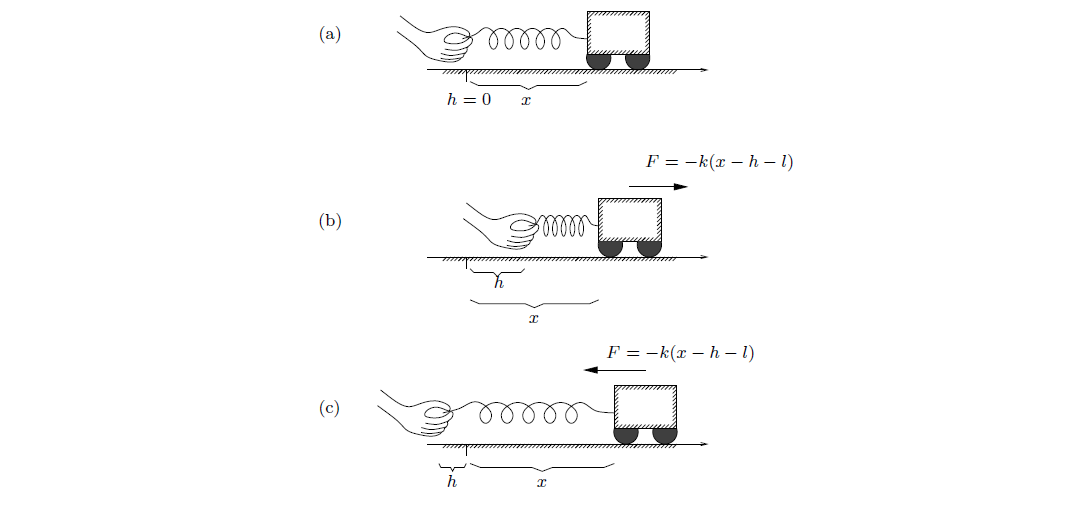
\includegraphics[scale=0.5]{imagem}
\caption{Sistema massa-mola com extremo variável: (a) na posição de equilíbrio ($x - h = l$), (b) com a mola contraída ($x - h < l$), e (c) com a mola estendida ($x - h > l$), onde $l$ é o comprimento de equilíbrio da mola}
\label{fig:inicial}
\end{figure}


\par
Fazendo-se uma substituição de variáveis, obtém-se duas equações diferenciais de primeira ordem:
\begin{equation}
\label{EDO}
v=x'\\
v'=k\frac{h+l-x}{m}
\end{equation}
onde $v$ é a nova variável, que representa, fisicamente, a velocidade.
Vale a pena notar que, muitas vezes, a equação de sistemas oscilatórios é descrito como:
\begin{equation}
    \frac{d^2x}{dt^2}+\omega_{0}^2x=0
\end{equation}
onde $\omega_{0}=\sqrt{\frac{k}{m}}$ é a frequência natural do sistema. Se a frequência da força externa $\omega$ for igual a $\omega_{0}$, ocorrerá o fenômeno de ressonância em oscilações forçadas. Esta condição fornece:
\begin{equation}
\label{omega}
    \omega_{0}=\omega=\sqrt{\frac{k}{m}}
\end{equation}

\section{Metodologia Numérica}
\subsection{Discretização do modelo matemático}
A discretização do problema será feita através do Método Implícito de Euler. Então seja $t_0$ o instante inicial de estudo, e $t_f$
o tempo final, e $n$ o número de divisões do intervalo $I=[t_0,t_f]$, tem-se:
\begin{equation}
\Delta t=\frac{t_f-t_0}{n}
\end{equation}
\par
O Método Implícito de Euler para um vetor de EDO é, para duas funções $x$ e $y$:
\begin{equation}
\label{MIE}
\left(\begin{array}{c}
x_{k+1}\\
y_{k+1} \end{array}\right) = \left( \begin{array}{c}
x_k+\Delta t g_{1}(t_{k+1},x_{k+1},y_{k+1})\\
y_k+\Delta t g_{2}(t_{k+1},x_{k+1},y_{k+1})
\end{array}\right)
\end{equation}
\par
Desta  forma, o sistema massa-mola fornece a seguinte equação, partindo de (\ref{MIE}), substituindo-se as funções de derivada de acordo com a equação (\ref{EDO}):
\begin{equation}
\left(\begin{array}{c}
x_{k+1}\\
v_{k+1} \end{array}\right) = \left( \begin{array}{c}
x_k+\Delta tv_{k+1}\\
v_k+\Delta t(k\frac{(-x_{k+1}+h+l)}{m})
\end{array}\right)
\end{equation}
\par
Observa-se que será necessário o uso de métodos de zeros de funções, adaptados para vetores de duas dimensões. Estes métodos se utilizam da matriz jacobiana, que é utilizada para encontrar $x_{k+1}$ e $v_{k+1}$. Nesse ponto entra o Método de Newton.
\par
Uma vez que o problema foi discretizado, uma nova etapa se fez necessário: encontrar valores futuros (em passos de tempos futuros) das variáveis de integração. 
\par
Sejam duas novas funções definidas como:
\begin{equation}
\begin{split}
f_{1}(x_{k+1},v_{k+1})=x_{k}+\Delta t v_{k+1}-x_{k+1} \\
f_{2}(x_{k+1},v_{k+1})=v_{k}+\Delta t(\frac{k(-x_{k+1}+h+l)}{m})-v_{k+1} 
\end{split}
\end{equation}
\par
Estas funções reduzem o problema a encontrar zero de funções. Neste ponto, entra o Método de Newton.
\par
Lembrando que a Matriz Jacobiana $2x2$ é da forma:
\begin{equation}
J(f_{1}(x,v),f_2(x,v)) = \left[ 
  \begin{tabular}{cc}
  $\frac{\partial f_{1}}{\partial x}$ & $\frac{\partial f_{1}}{\partial v}$  \\
  $\frac{\partial f_{2}}{\partial x}$ & $\frac{\partial f_{2}}{\partial b}$  \\
  \end{tabular}
\right]
\end{equation}
\par
Obtém-se para este problema:
\begin{equation}
J(f_{1}(x_{k+1},v_{k+1}),f_2(x_{k+1},v_{k+1})) = \left[ 
  \begin{tabular}{cc}
  -1 & $\Delta t$  \\
  $\frac{-k\Delta t}{m}$ & -1  \\
  \end{tabular}
\right]
\end{equation}
\par
Será preciso inverter a matriz, como é exigido pelo método. Assim teremos a inversa da matriz Jacobiana:
\begin{equation}
J^{-1} = \frac{1}{1+\frac{k\Delta t^2}{m}}\left[ 
  \begin{tabular}{cc}
  -1 & $\frac{k\Delta t}{m}$  \\
  $-\Delta t$ & -1  \\
  \end{tabular}
\right]
\end{equation}
\par
Finalmente, o problema é resolvido numericamente, realizando-se as seguintes iterações, cujo índice é $i$:
\begin{equation}
\left[ 
  \begin{tabular}{c}
  $x_{k+1}^{i+1}$  \\
  $v_{k+1}^{i+1}$  \\
  \end{tabular} \right]=\left[
  \begin{tabular}{c}
  $x_{k+1}^{i}$  \\
  $v_{k+1}^{i}$  \\
  \end{tabular}\right] -J^{-1}\left[ 
  \begin{tabular}{c}
  $f_{1}(x_{k+1}^{i},v_{k+1}^{i})$ \\
  $f_{2}(x_{k+1}^{i},v_{k+1}^{i})$ \\
  \end{tabular}
\right]
\end{equation}

A cada iteração $k$ encontra-se através de iterações $i$ os zeros das funções para o próximo valor a cada tempo $t$.
No nosso caso consideramos como condição de parada uma quantidade iteração $i=100$ garantindo a não propagação de erro para o Método Implícito.

\section{Resultados}
\subsection{Escolha de parâmetros do problema}
Um problema puramente genérico não pode ser resolvido numericamente. Por este motivo, serão escolhidos valores para todas as constantes do sistema massa mola.
\par
O caso de interesse é o de oscilação ressonante. Para garantir que a ressonância ocorra, basta atender à equação (\ref{omega}).
\par
    \begin{tabular}{|p{3cm}|p{3cm}|}
        \hline
        \multicolumn{2}{|c|}{Definição de constantes}\\
        \hline
        Constante & Valor\\
        \hline
        k & 1 kg/$s^{2}$  \\
        \hline
        m & 1 kg\\
        \hline
        $\omega$ & 1 rad/s\\
        \hline
        h(t) & $h_{0}sin(\omega t)$ cm\\
        \hline
        $h_{0}$ & 0,1 m\\
        \hline
        L & 1 m\\
        \hline
    \end{tabular}


\subsection{Solução}

Utilizando-se do Método de Newton, foi escrito um programa em C, a partir dos valores das constantes, mostrados na tabela. Também foram considerados os valores de $t_{0}=0$, $t_{f}=60$, $v_{0}=0$ e $x_{0}=0.9m$, como parâmetros de condição inicial, e $n = 2^{10}$ como o número de partições de integração. O programa forneceu os seguintes gráficos, que representam a solução.
\par

\begin{figure}[h]
\begin{subfigure}{0.5\textwidth}
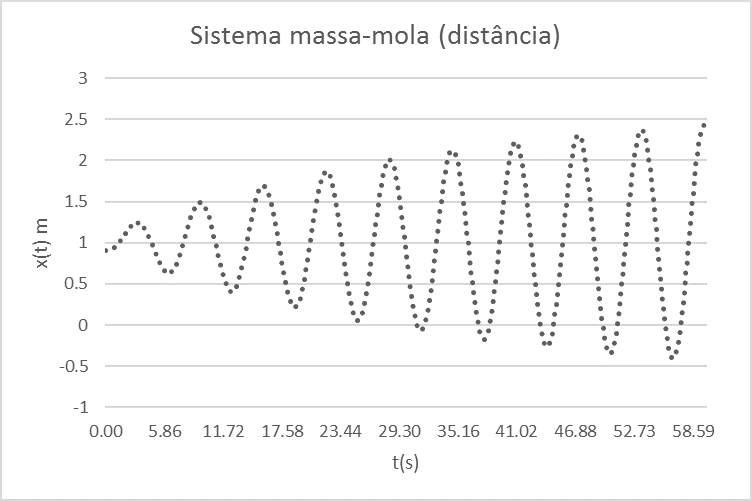
\includegraphics[width=1.0\linewidth, height=6cm]{distancia} 
\caption{Solução para distância, $\omega=1.0$}
\label{fig:subim1}
\end{subfigure}
\begin{subfigure}{0.5\textwidth}
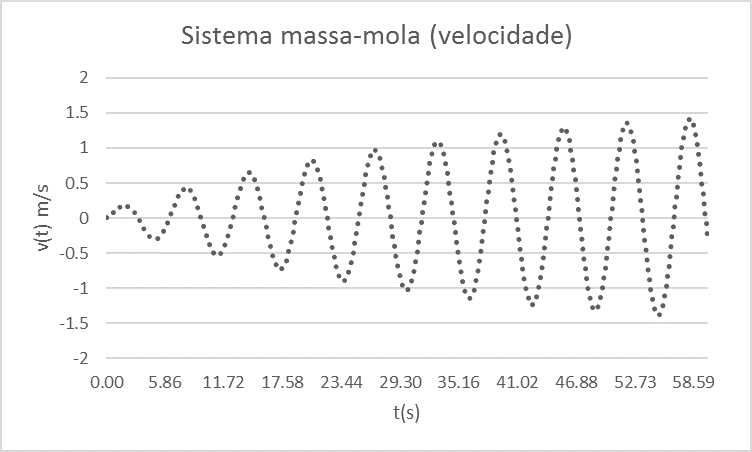
\includegraphics[width=1.0\linewidth, height=6cm]{velocidade}
\caption{Solução para velocidade, $\omega=1.0$}
\label{fig:subim2}
\end{subfigure}
\begin{subfigure}{0.5\textwidth}
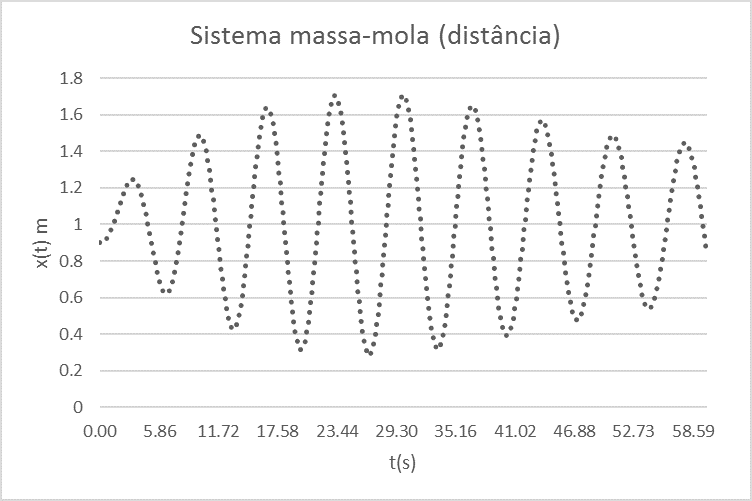
\includegraphics[width=1.0\linewidth, height=6cm]{distancia2} 
\caption{Solução para distância, $\omega=0.9$}
\label{fig:subim3}
\end{subfigure}
\begin{subfigure}{0.5\textwidth}
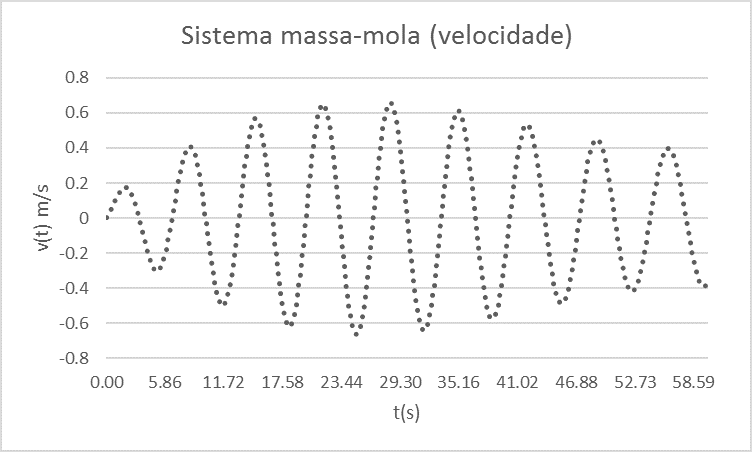
\includegraphics[width=1.0\linewidth, height=6cm]{velocidade2}
\caption{Solução para velocidade, $\omega=0.9$}
\label{fig:subim4}
\end{subfigure}
\caption{Soluções encontradas pelo Método de Newton.}
\label{fig:image2}
\end{figure}
\clearpage
\par
Assim, temos, a partir das soluções, resultados numéricos, na qual podemos ver o comportamento ressonante do sistema. Vale notar que, a medida que $\omega$ se aproxima de $\omega_{0}$ (ver equação (\ref{omega})), a amplitude de oscilação aumenta, de acordo com o comportamento esperado do movimento ressonante. Estes e outros resultados podem ser encontrados no livro Rosa \cite{Rosa}, pág. 135, fig 3.2.


\section{Conclusões} 
O estudo do sistema massa-mola fornece a equação que descreve a forma como a massa se descola, nas condições do problema. As equações deste sistema permitem que seja encontrada uma relação entre a frequência de oscilação da massa e da força externa. A análise numérica presente neste trabalho mostrou, através dos gráficos, que, quando estas frequências se igualam, o sistema entra em ressonância, resultando numa amplitude crescente com o passar do tempo.
\par
Os problemas físicos, como condições de segurança de uma ponte de grande porte, por exemplo, devem levar em conta os resultados obtidos neste trabalho, pois a ressonância, nesse caso, é algo indesejado e perigoso, sendo necessário conhecer as condições que implicam em ressonância, assim como os resultados de um sistema ressonante.
\par
Outros casos, como na receptação de ondas eletromagnéticas, necessitam das equações aqui estudada, pois, para receber corretamente uma certa informação, é preciso que o receptor entre em ressonância com o emissor.
\par
A ressonância é encontrada em diversas áreas, e cada uma a enxerga de formas diferentes. Portanto, é preciso ter conhecimento das equações solução do sistema massa-mola, assim como dos resultados gráficos e numéricos, para as diferentes condições possíveis (com ou sem ressonância).



\printbibliography[heading=bibintoc]
\end{document} %finaliza o documento



